\chapter[Towards an extensible measurement of metadata quality]{Towards an extensible measurement of metadata quality\footnote{This chapter is an extended version of the paper \cite{kiraly2017}.}}

\section{Introduction}

In the literature about metadata quality measurement\footnote{The most current bibliography of the topic is the collaborative Metadata Assesment Zotero group library created by the DLF AIG Metadata Working Group (\url{http://dlfmetadataassessment.github.io/}). Available at \url{https://www.zotero.org/groups/metadata_assessment}.} it is rare that the authors give any hint about their implementation methods or give a reference to their source codes. 
Thus -- since as readers of these papers we lack the opportunity of studying the implementation details --, we are forced to assume that these projects aimed to measure one specific dataset based on a particular metadata schema. When I started my research, it was an important aspect that the tool I design (called as the time being ``Metadata Quality Assurance Framework''\footnote{Background information, documentation and source codes are available from \url{http://pkiraly.github.io/}.}) should work together with different metadata schemas and formats.

The quality assessment process has three phases:

\begin{enumerate}
\item Measuring individual metadata records
\item Analyzing the results with statistical methods to get metrics of the dataset
\item Reporting results
\end{enumerate}

The results of the first phase are table-like data structures containing mostly numerical values. Since these type of results are very similar for different metadata schemas, the second phase can already be handled in general way with statistical and data science methods. The first step should however be investigates further. The basic process of measuring is the following: the tool takes a record as a formatted string (in JSON or XML format), addresses individual parts to check their existence, cardinality or other properties (different features of their content) and returns the results of these checks (typically in numerical form). If one would like to abstract this process she should figure it out how to list and access individual parts of the metadata record, and she also should provide schema-independent measurement methods.

This chapter will describe the steps I took so far to support this abstraction, which enables us to measure different metadata collections with a single tool.

\section{Types of measurement}

The main types of data quality measurement the tool can run on metadata records are the following:

1. General structural and semantic metrics. These measurements are the most well known in the literature, and following the seminal articles \cite{bruce-hillmann2004, ochoa-duval2009} several projects reported to measure
the metrics of completeness (the existence of the defined fields in the records), accuracy (comparison of a full data object and its metadata), conformance to expectations (schema rule validation and information value), logical consistency and coherence, accessibility (how easy is to understand the text of the record), timeliness (the metadata quality change over time) and provenance (the relationship between other metrics and the creator of the data).

2. Support of functional requirements. Each data schema is created for supporting a set of functionalities, such as searching, identifying or describing objects. The data elements support one or more of these functionalities, and their existence and content has an impact of these functionalities. An example: a timeline widget expects a specific date format; if the field value is in another format the widget will ignore it. This family of metrics gives measures the scale of support of the functional requirement. To apply these metrics a functional requirement analysis of the data schema should be conducted, and mapping the individual data elements (classes and properties) to the functionalities. The result will be a report which tells how the data support the intended functions. Following the terminology established in \cite{gavrilis2015} I call these scores `sub-dimensions'. In the Europeana Data Quality Committee Valentine Charles and Cecile Devarenne defined a number of sub-dimensions (such as searchability, descriptiveness, identification, contextualization, browsing etc.) which could be re-used in other metadata domains.

3. Existence of known data patterns. These are schema- and domain-specific patterns which occurs frequently in the datasets. There are good patterns which detect good data creation practices, and anti-patterns, which should be avoided (such as data repetition, meaningless data etc.). For some domains there are existing pattern catalogs (e.g. the Europeana Data Quality Committee works on a Europeana specific pattern catalog, while \cite{suominen2012} examined three SKOS validation criteria catalogs).

4. Multilinguality. RDF provides an easily adaptable technique to add a language tag to literal values, and multilinguality has become a key aspect in the Linked Open Data world. In cultural heritage databases the translation of the descriptive fields (such as title, description) might be quite a resource-intensive task. On the other hand reusing existing multilingual dictionaries for subject headings is a relatively simple and cheap process. On the measurement side the nice thing is that generally the multilingual layer in metadata schemas (even in those not built on top of RDF) are similar, so the implementation can be abstracted. The big problem is how to handle the biases generated by the different cardinality and importance of the data elements. Imagine that we have a subject heading which is accessible in several language, but it is attached to a great portion of records, so its information value or distinctive power is low. See more about multilinguality in \cite{stiller-kiraly2017}.

The common point in these metrics is that they can be implemented as generic functions where input parameters are specific elements of a data schema. The functions themselves should not know about the details of the schema; that is to say they should be schema-independent. In other words: the only thing need to be created on a schema by schema basis is a method which takes care of mapping the schema elements and measurement functions and feeds these generic functions with the appropriate metadata elements.

Note: based on these metrics on the following, analytic phase a mathematical model have to be created that generates one or more top level data quality score for the record; this chapter does not discuss this phase.

\section{Mapping schema and measurements}

A metadata schema describes the structure of the record, and optionally gives us constraints upon the values of the fields. In order to measure the metadata quality various pieces of information are needed about the schema:

\begin{itemize}
 \setlength{\parskip}{0pt}
 \setlength{\itemsep}{0pt plus 1pt}
\item What are the fields to be analysed?
\item Are there any special properties of a field (e.g. mandatory or optional, repeatable, content-related constraints, special format)?
\item Are there fields the tool has to extract to identify the record or a subset of the collection?
\item Are there field groups which can behave in special way? (For example: if a record must have at least a title or an alternative title, the tool should group these together, and when checking the mandatory elements it should return true if at least one element of the group exists. Conversely, disjoint fields (which are mutually exclusive) should be checked that only one one of them is available in the record, but never more.)
\end{itemize}

In the previous section I mentioned that I had to create a mapping mechanism which dispatches the elements of the metadata record to different measurement functions. In the first iteration of the Metadata Quality Assurance Framework I have created an abstract concept of the schema, which lists the metadata elements needed for the quality analyses. Each element has a name, an address with which its occurrences can be found within the record, and different properties which denote its role in a particular function (for example the list of sub-dimensions it is part of, the list of field groups, whether it might have language annotation etc.). The mapping supports parent-children relationship, so the functions can recurse down the hierarchy.

A prerequisite for measuring information value is a searchable index, which I implemented with Apache Solr. In the framework, metadata fields are accordingly mapped to Solr field names.

In this mapping the tool records all information about the metadata schema which is necessary for the measuring. At time of writing the manifestation of this mapping is a Java class.\footnote{Such as \url{https://github.com/pkiraly/metadata-qa-api/blob/master/src/main/java/de/gwdg/metadataqa/api/schema/EdmOaiPmhXmlSchema.java}} To run the measurement on a new schema, one should create first this mapping object. In the future I will create user friendly interfaces (web-based editorial form and XML/RDF annotations) which are more familiar tools for the intended audience, the community of metadata experts.

\subsection{Addressing elements}

An important part of schema handling is how it addresses the particular parts of the record. In the XML world XPath\footnote{XML Path Language (XPath). Version 1.0. W3C Recommendation 16 November 1999 (Status updated October 2016). \url{https://www.w3.org/TR/xpath/}} provides with a standard way to solve this problem. The current version of the Metadata Quality Assurance Framework (version 0.4) supports only JSON records, so it makes use of a similar tool, JsonPath\footnote{Stefan Goessner: JSONPath --- XPath for JSON. \url{http://goessner.net/articles/JsonPath/}. Actually it uses its Java port, the Jayway JsonPath available at \url{https://github.com/jayway/JsonPath}} which has a different syntax, but offers the same functionality. To illustrate it here is an example for the Europeana Data Model (EDM) metadata schema\footnote{The Europeana Data Model Documentation is available at \url{http://pro.europeana.eu/share-your-data/data-guidelines/edm-documentation}}:

\begin{lstlisting}[caption=A JSON path example]
$.['ore:Proxy']
  [?(@['edm:europeanaProxy'][0] == 'false')]
  ['dc:title']
\end{lstlisting}

This expression addresses the dc$:$title field instances of the ore$:$Proxy part in which the value of the first edm$:$europeanaProxy instance is 'false'.

\begin{lstlisting}[caption=An excerpt of an EDM metadata record]
{
  "ore:Proxy": [
    {
      "edm:europeanaProxy": ["false"],
      "dc:title": [
        {
          "@lang": "de",
          "#value": "Pyrker-Oberwart, Johann Ladislaus"
        }
      ],
      ...
    },
    {
      "edm:europeanaProxy": ["true"],
      ...
    }
  ]
}
\end{lstlisting}

Here you can see that the ore$:$Proxy is a list of two objects. The first one's edm$:$europeanaProxy is `falue', the second one's is `true'. Since we are looking for the the object with the `false' value, we get the first. It has a `dc$:$title' property. The return value will be the Java representation of the following JSON string:

\begin{lstlisting}[caption=The selected part of the record]
[
  {
    "@lang": "de",
    "#value": "Pyrker-Oberwart, Johann Ladislaus"
  }
]
\end{lstlisting}

In this example an absolute path is shown, which searches from the root of the record, but since the schema abstraction supports parent-child relations, relative paths can be used as well.

\subsection{Flexible and configurable measurements}

\subsubsection{The overall picture}

The system's central entry point is the CalculatorFacade (or its extension). It provides us with a number of configuration options. The most important one is the registration of the schema mapping. Based on the settingsin the schema mapping it prepares the measurement classes for running. When it is ready to run the process passes every record to the measure() method. It accepts the metadata record as a JSON string, runs all the measurements which have been configured, and returns a CSV representation of the result of the metrics. As indicated by the name it is just a Facade object\footnote{See \url{https://en.wikipedia.org/wiki/Facade_pattern}}: it only coordinates the process, the actual measurements are done by the individual 'calculators' (the generic schema-agnostic functions I mentioned above). These all implement the Calculator interface, and they have three important methods. The 'measure()' method accepts a cacheable representation of the metadata record and performs the measurement. The 'getCsv()' method returns the result of the measurement, while 'getHeader()' method returns a list of the column names for the CSV row. The cacheable representation is a special object. It contains the full record or a part thereof, applies the JsonPath expressions, and transforms the resulting object into a uniform Java object, which provides a simplified DOM-like interface. In this fashion the Calculators can access the values in a generalized way, and can reuse the already-processed parts from the cache. Retrieving the parts of the record is computationally expensive: one part might participate in multiple measurements, but this way the tool has to retrieve it only once.

Each calculator implements one or more metrics. Since at run-time (in the measuring phase) they can not get extra arguments, if a calculator has conditional steps depending on properties which are not part of the schema, they should be configured ahead of the measuring phase via the CalculatorFacade's 'configure()' method. For example the 'MultilingualitySaturationCalculator' can emit its results in either simple and complex form, depending on the 'resultType' setting. The client should decide the format before running the measurement, and set the appropriate one in the Facade class.

This way the CalculatorFacade are extensible, and one can write additional Calculators. The tool currently provides all Calculators required for our current research.

\subsubsection{Metadata problem patterns}

Problem patterns are known issues in the metadata record instances. In case of Europeana Timothy Hill and Hugo Manguinhas have led the initiative to collect all those problems\footnote{Data Quality Committee: Problem Patterns. Available at \url{http://bit.ly/2jIXQGU}}. They categorized the problems into several types, such as duplicate or redundant information, irrelevant information (such as non-meaningful titles, e.g. "unknown title"), missing or incomplete information, misuse of fields, just to name a few.

The current implementation of the problem catalog measurement has been done based on the Observer design pattern \footnote{\url{https://en.wikipedia.org/wiki/Observer_pattern}}. There is a central class --- ProblemCatalog\footnote{\url{https://github.com/pkiraly/metadata-qa-api/blob/master/src/main/java/de/gwdg/metadataqa/api/problemcatalog/ProblemCatalog.java}} --- which implements the Calculator interface, so it has a 'measure()' method. This class acts as the observable subject, and it notifies its subscribers (the observers) when they have to measure a new record. Each individual problem is associated with a distinct class (a ProblemDetector\footnote{See for example the 'EmptyStrings' class which detects empty strings in field instances: \url{https://github.com/pkiraly/metadata-qa-api/blob/master/src/main/java/de/gwdg/metadataqa/api/problemcatalog/EmptyStrings.java}}), which implements the Observer interface, and accordingly has a method called 'update()'. It has two parameters: the metadata record, and a variable which is a collector of the measurement results. In this case the result should be a number: how many times the pattern occurs in the record. When the measure is started, the ProblemCatalog class creates a collector for these results, and the client (the facade class) will retrieve it when the measurement is done.

The ProblemCatalog class has 'addObserver()' method to register the subscribers, which should be done at the central facade class at configuration time.

For detecting new problems one has to create new ProblemDetectors and register them in the central CalculatorFacade.

\subsection{Extensions and APIs}

The current Java APIs are defined in a core library (metadata-qa-api) which contains the workflow governing mechanism, and the general schema-agnostic functionalities. There is an extension of this API, called 'europeana-qa-api' that contains the Europeana-specific measurement and facade. These libraries are published in the central Maven repository\footnote{\url{http://mvnrepository.com/artifact/de.gwdg.metadataqa}}, so any further extension can add these into its dependency tree in the local Maven configuration file (pom.xml) as

\begin{lstlisting}[caption=Including the Java libraries into other project]
<dependencies>
  <dependency>
    <groupId>de.gwdg.metadataqa</groupId>
    <artifactId>metadata-qa-api</artifactId>
    <version>0.4</version>
  </dependency>
  <dependency>
    <groupId>de.gwdg.metadataqa</groupId>
    <artifactId>europeana-qa-api</artifactId>
    <version>0.4</version>
  </dependency>
  ...
</dependencies>
\end{lstlisting}

I have created two clients for the Java APIs: the first enables measurement with the popular Big Data analytics tool Apache Spark; the second one provides us with a REST interface.

\subsubsection{Big Data analysis}

Apache Spark is an extremely efficient tool for batch processing of huge datasets (the Europeana dataset is more than 400 GB). Combined with Apache Hadoop's distributed file system it can be run either on a single machine or in a distributed computing environment. The users can specify the details of allowable resource usage (number of CPUs, memory usage, etc.) and it comes with a web based monitoring tool. In the file-based workflow, Spark reads and processes lines one by one; it requires us to store one record per line (however Spark also supports different other data sources such as NoSQL databases, where this constraint does not exist). In our Spark based client the result is stored as CSV files.

\subsubsection{Data analysis with REST APIs}

The REST interface provides two kinds of API: a simple Record API, which runs the measurement on individual records and returns a CSV or JSON response, and another one which is called Workflow API and enables a full measurement workflow.

\begin{lstlisting}[
  % one can adjust spacing here if required
  % aboveskip=2.5\baselineskip,
  % belowskip=-.8\baselineskip,
  caption={Quality measurement of a single record REST API response},
  label=code:single-record-api-json-response,
  language=Bash,
  float]
GET /07602/696BE60475DFAF290B7CD7759E840CD4FFF86E24.json

{
  "existingFields":[
    "edm:ProvidedCHO/@about", "Proxy/dc:title", "Proxy/dc:creator",
    "Proxy/dc:publisher", "Proxy/dc:type", "Proxy/dcterms:spatial",
    ...
  ]
  "emptyFields":[],
  "labelledResults":{
    "fields":{
      "recordId":"/07602/696BE60475DFAF290B7CD7759E840CD4FFF86E24",
      "dataset":"07602_Ag_IT_Culturalitalia_RegioneMarche",
      "dataProvider":"Regione Marche / SchedeS:AN" },
      "completeness":{
        "TOTAL":0.542857, "MANDATORY":1.0, "DESCRIPTIVENESS":0.454545,
        ...
      },
      "existence":{
        "edm:ProvidedCHO/@about":true, "Proxy/dc:title":true,
        "Proxy/dcterms:alternative":false, "Proxy/dc:description":false,
        ...
      },
      "cardinality":{
        "edm:ProvidedCHO/@about":1, "Proxy/dc:title":1,
        "Proxy/dcterms:alternative":0, "Proxy/dc:description":0,
        ...
      },
      "uniqueness":{
        "dc:title:sum":0.001084, "dc:title:avg":1.807687E-4,
        "dcterms:alternative:sum":0.0, "dcterms:alternative:avg":0.0,
        "dc:description:sum":0.0, "dc:description:avg":0.0
      },
      "problemCatalog":{
        "LongSubject":1.0, "TitleAndDescriptionAreSame":0.0,
        "EmptyStrings":0.0
      },
      "languages":{
        "Proxy/dc:title":{ "_0":1 }, 
        "Proxy/dcterms:alternative":{ "_1":1 },
        ...
      }
    },
    "termsCollection":{
      "dc:title":[
        {"term":"ancona", "tf":1, "df":12388, "tfIdf":8.072328-5},
        {"term":"carta", "tf":1, "df":87048, "tfIdf":1.148791-5},
        ...
      ],
      "dcterms:alternative":[],
      "dc:description":[]
    }
  }
}
\end{lstlisting}

Listing \ref{code:single-record-api-json-response} shows a formatted representation of the Record API call. It accepts two parameters, the record ID, and the format (either as JSON or CSV) as file extension. The result contains all the measurement results for an individual record. At time of writing the measurements are existence, cardinality, uniqueness, problem catalog and languages. The languages part contains pairs of languages and their count for each fields. There are three special codes to encode cases where there is no language annotation:

\begin{itemize}
  \setlength{\parskip}{0pt}
  \setlength{\itemsep}{0pt plus 1pt}
  \item \_0: no language tag specified
  \item \_1: the field is missing (the very same information that of field existence metric)
  \item \_2: the field is a resource (it contains a URL or tagged as resource)
\end{itemize}

The user interface's record level display is based on the Record API.

\begin{figure}
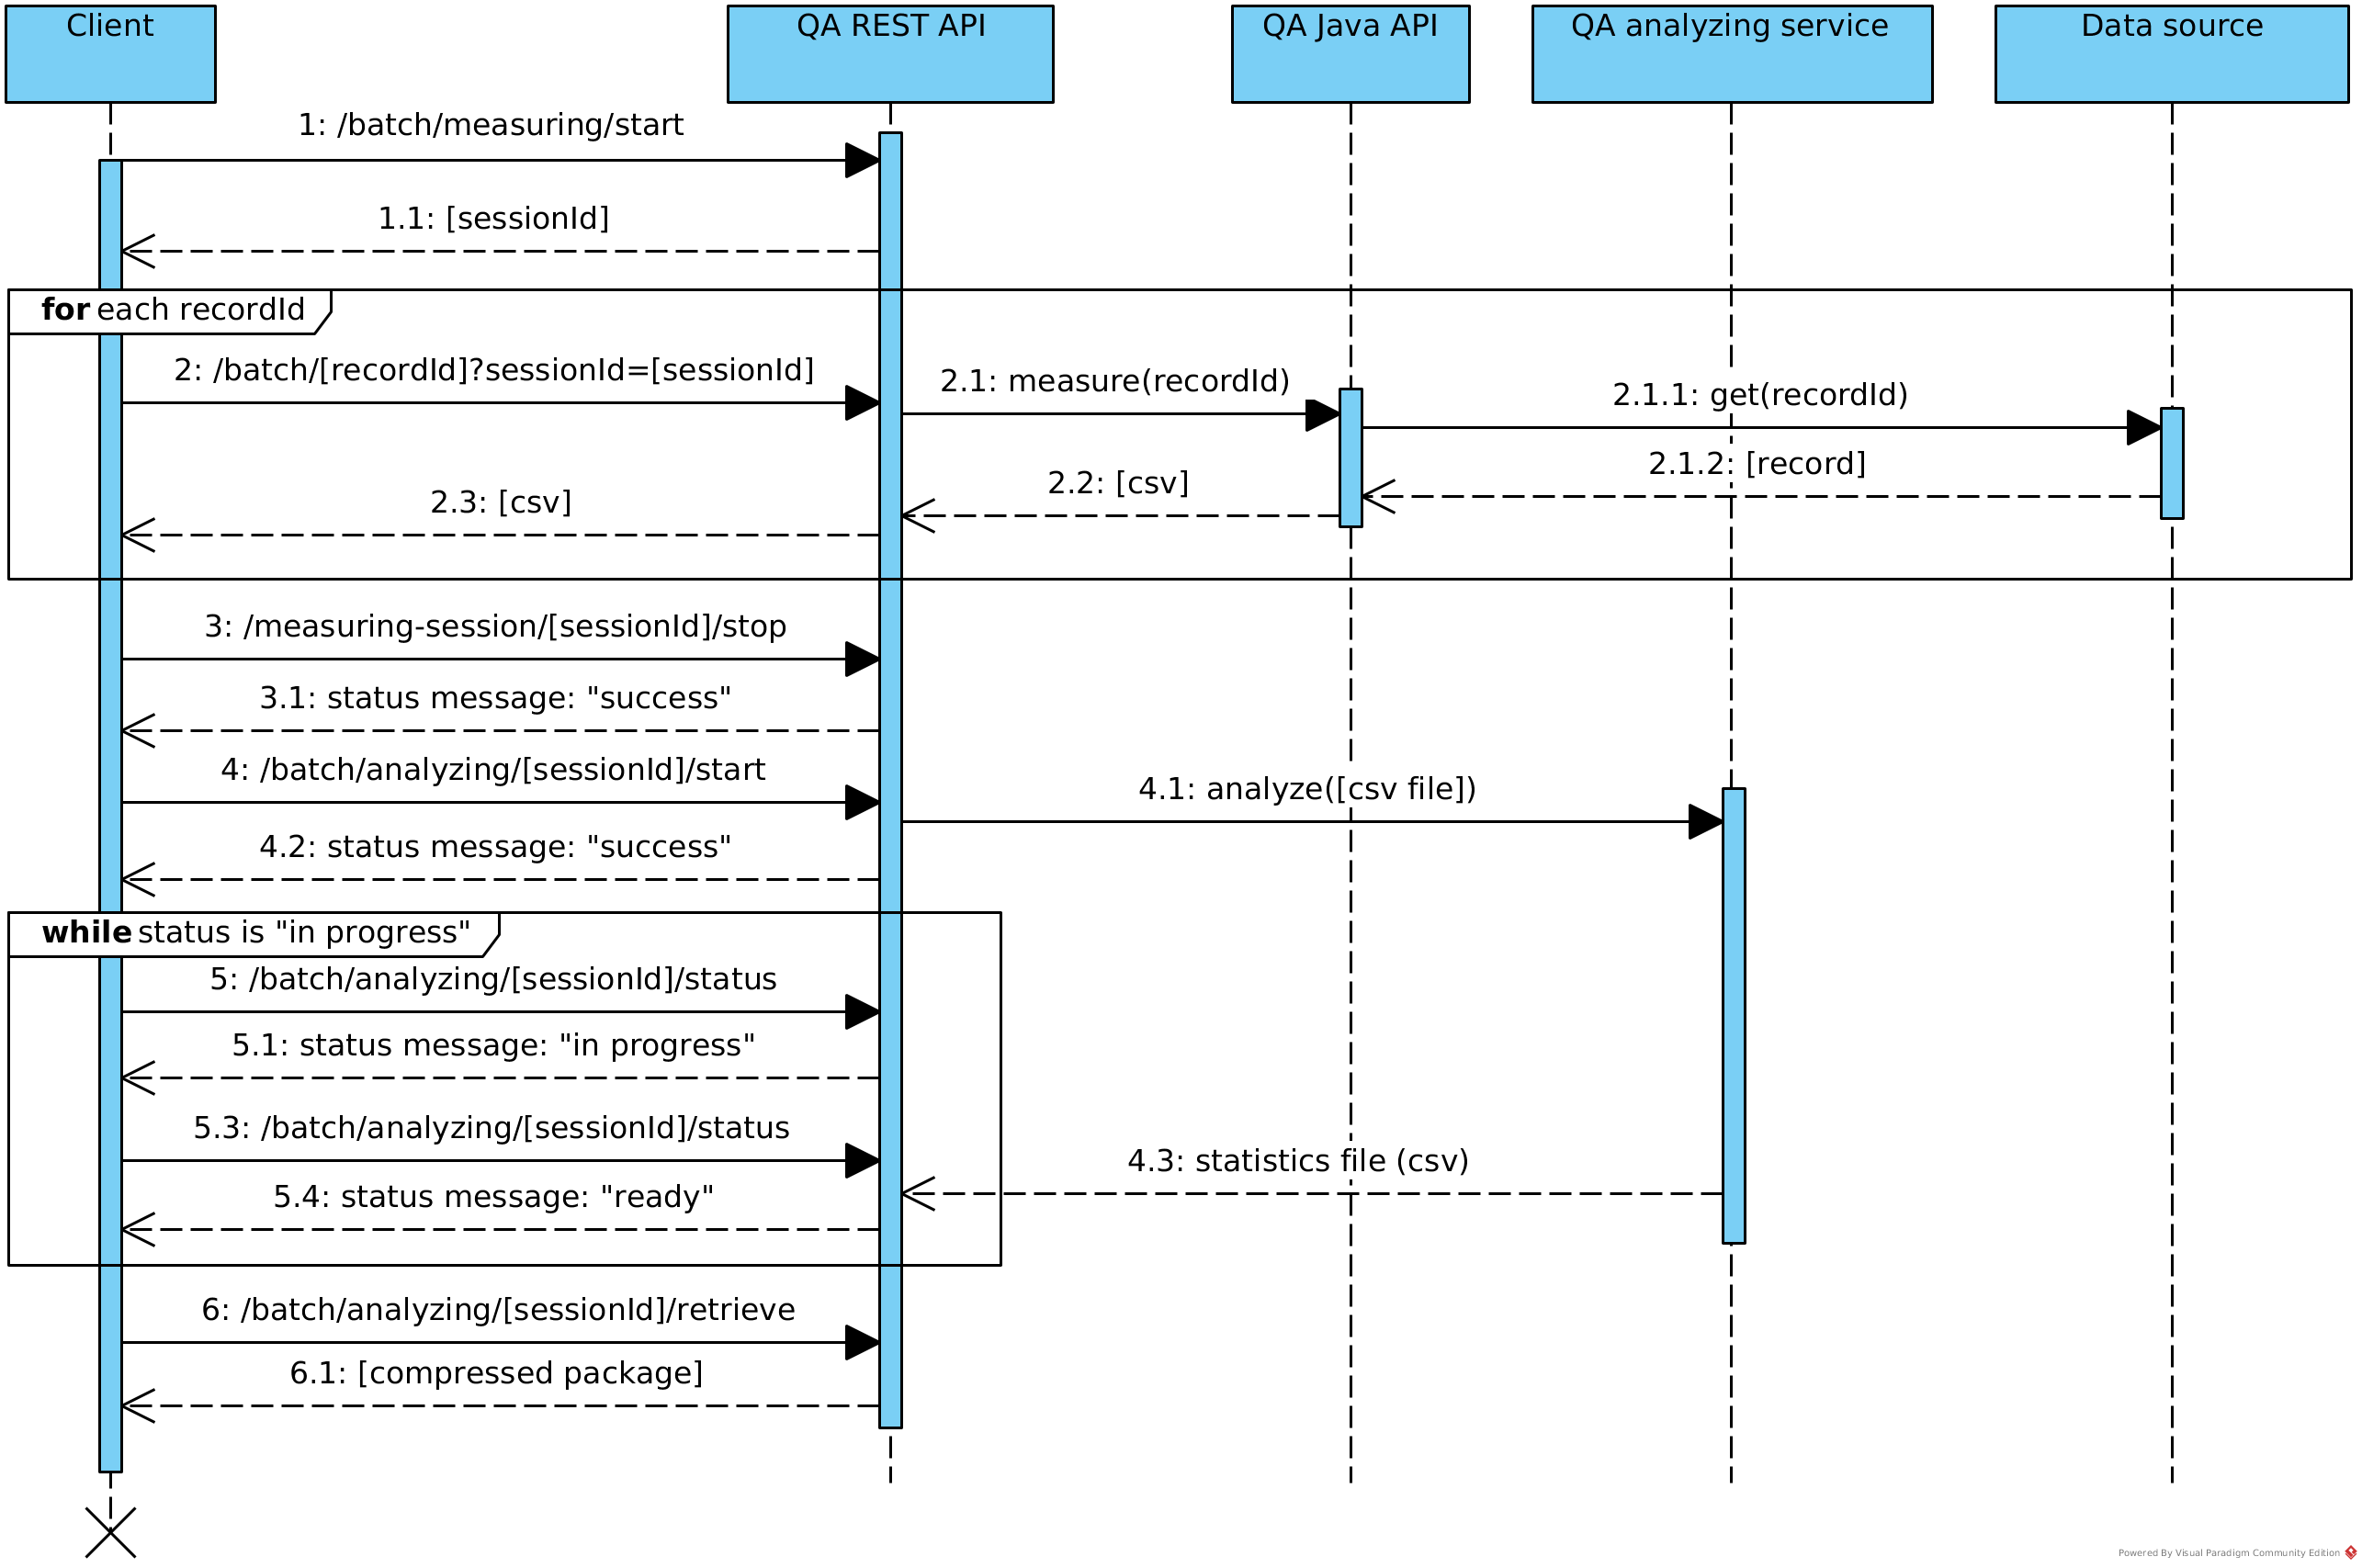
\includegraphics[width=\textwidth]{images/chapter05/QA-REST-API-interactions.png}
\caption{Processing time per records with different settings}
\label{figure:workflow-api}
\end{figure}

The Workflow API supports the whole life cycle of the metadata quality measurement process, so it measures individual records, then analyze them by running statistical functions on aggregated metrics. The full workflow is depicted by Figure \ref{figure:workflow-api}. 

First, the client initializes a session, to which the server returns a session identifier which should be used during the whole workflow. Then client submits record IDs one by one. The server is responsible for storing the results in a CSV file, but it also returns a CSV row for each record call, same way as the Record API does. Once all records were measured, the client stops the measuring part, and starts the analysis part, in which the server calls the external analyzer (either a R script or a Spark based analysis process) to produce a report containing the result of the statistical analysis and (optionally) generated images files. This process is time consuming, and the client can repeatedly ask for the status of the process. The server reports if the process is ``in progress'' or ``ready''. When it is finished, the client can retrieve the result as a zipped package. This process is very useful if the client would like to check only a part of the whole collection. Combined with other tools (e.g. with a search API) it is possible to select the IDs of a subset -- for example the newly ingested records, or a specific result set.

The main reason for creating REST APIs is that this way the back end functionalities of the framework became interoperable: the metrics could be reused in the client's own existing systems.

\section{Conclusions and future works}

In this chapter I showed the most important technical requirements of an extensible metadata quality assessment framework. I discussed the first phase of the metadata quality analytics workflow only, the measurement part. It can ingests different metadata schemas, but emits numerical, tabular data in a standardised form. The statistical analysis, and the reporting based on this, and do not require the same abstracting approach as the first step.

I showed the main characteristics of the metadata quality metrics and the metadata schema, then how to map schema features to measurement functions and how to address internal parts of a metadata record. I discussed the relevant design decisions of our implementation, and highlighted the parts which should be extended if one adapts the method for another metadata schema. Finally I described the APIs of the system.

By the time of writing no other projects started to use this framework, so I do not have real external feedback about the flexibility of the framework. Our own experiments were based on two metadata schema: Europeana Data Model (EDM) and MAchine Readable Catalog (MARC21) --- both of which have relatively simple structures. I expect that every new metadata schema will raise at least some new requirements, and only after having successfully dealt with a variety of schemas I will be in a position to release a 1.0 version of the tool. The level of schema abstraction is adequate for current purposes, but I anticipate the addition of several new features in the future. I am constantly looking for collaborating partners to try this approach on new schemas and in different IT environments. Starting and continuing discussions with organizations having similar approaches and requirements in the realms of digital libraries, the semantic web, digital humanities, and learning objects, and learning from each other will be a crucial aspect of creating a truly interoperable framework.

\section{Acknowledgments}
I would like to thank Europeana and GWDG for providing computational environment for this research. For this research Cecile Devarenne and Yorgos Mamakis (Europeana) for giving suggestions regarding to the Workflow API, and all the members of the Data Quality Committee\footnote{\url{http://pro.europeana.eu/page/data-quality-committee}} for their work, and Timothy Hill for language-related suggestions.

% \bibliographystyle{acm}
% \bibliography{bibliography-for-papers}
